\documentclass[
12pt,
a4paper,
pdftex,
czech,
titlepage
]{report}

\usepackage[czech]{babel}
\usepackage[utf8]{inputenc}
\usepackage{lmodern}
\usepackage{textcomp}
\usepackage[T1]{fontenc}
\usepackage{amsfonts}
\usepackage{titlesec}
\usepackage{listings}
\usepackage{graphicx}

\titleformat{\chapter}
  {\normalfont\LARGE\bfseries}{\thechapter}{1em}{}
\titlespacing*{\chapter}{0pt}{0ex plus 1ex minus .2ex}{2.0ex plus .2ex}

\begin{document}

\begin{titlepage}
	\vspace*{-2cm}
	{\centering
\includegraphics[scale=0.3]{img/FAV_logo_jvs.jpg}\par}
	\centering
	\vspace*{2cm}
	{\Large Semestrální práce KIV/IR\par}
	\vspace{1.5cm}
	{\Huge\bfseries Implementace vlastního systému automatické indexace a vyhledávání dokumentů\par}
	\vspace{2cm}

	{\Large Jakub Hlaváč\par}
	{\Large A20N0050P\par}
	{\Large hlavja@students.zcu.cz\par}

	\vfill

	{\Large 14.\,04.\,2020}
\end{titlepage}

\tableofcontents
\thispagestyle{empty}
\clearpage

\chapter{Zadání}
\section{Popis zadání}
Cílem semestrální práce je naučit se implementovat komplexní systém s využitím hotových knihoven pro preprocessing. Vedlejším produktem bude hlubší porozumění indexerům, vyhledávacím systémům a přednáškám.
Systém po předchozím předzpracování zaindexuje zadané dokumenty a poté umožní vyhledávání nad vytvořeným indexem. Vyhledávání je možné zadáním dotazu s logickými operátory AND, OR, NOT a s použitím závorek. Výsledek dotazu by měl vrátit top x (např. 10) relevantních dokumentů seřazených dle relevance.
Semestrální práce musí umožňovat zaindexování dat stažených na cvičení (1. cvičení Crawler) a dat z portálu (složka TREC). Obě sady dat je možné zaindexovat nezávisle na sobě.
Semestrální práce musí umožňovat zadávat dotazy z GUI nebo CLI (command line interface), při zadávání dotazů je možné vybrat index a model vyhledávání (vector space model vs boolean model). Výsledky vyhledávání obsahují i celkový počet dokumentů, které odpovídají zadanému dotazu.
\label{minzadani}
\section{Minimální funkčnost}
\begin{itemize}
    \item tokenizace
    \item preprocessing (stopwords remover, stemmer/lemmatizer)
    \item vytvoření in-memory invertovaného indexu s oběma sadami dat
    \item tf-idf model
    \item cosine similarity
    \item vyhledávání pomocí dotazu vrací top x výsledků seřazených dle relevance (tj. vektorový model - vector space model)
    \item vyhledávání s pomocí logických operátorů AND, OR, NOT (booleovský model)
    \item podrobná dokumentace (programátorská i uživatelská)
    \item podpora závorek pro vynucení priority operátorů
\end{itemize}
\section{Nadstandardní funkčnost}
\begin{itemize}
    \item file-based index
    \item pozdější doindexování dat - přidání nových dat do existujícího indexu
    \item ošetření např. HTML tagů
    \item detekce jazyka dotazu a indexovaných dokumentů
    \item vylepšení vyhledávání
    \item vyhledávání frází (i stop slova)
    \item vyhledávání v okolí slova
    \item více scoring modelů
    \item indexování webového obsahu - zadám web, program stáhne data a rovnou je zaindexuje do existujícího indexu,
další předzpracování normalizace
    \item další předzpracování normalizace
    \item GUI/webové rozhraní
    \item napovídání keywords
    \item podpora více polí pro dokument (např. datum, od do)
    \item CRUD indexovaných dokumentů
    \item zvýraznění hledaného textu v náhledu výsledků
    \item dokumentace psaná v TEXu
    \item vlastní implementace parsování dotazů bez použití externí knihovny
    \item implementace dalšího modelu (použití sémantických prostorů)
\end{itemize}
\chapter{Aplikace}
Semestrální práce byla implementována jako webová aplikace a skládá se z BackEnd (Spring aplikace) a FrontEnd (apliakce Angular verze 11) části. Tyto dvě aplikace spolu komunikují pomocí nadefinovaného REST API.
\section{BackEnd}
Jedná se o standardní Spring aplikaci, která byla implementována pro Javu 11. Aplikace je rozdělena do několika balíků, které obsahují potřebné třídy.
\begin{itemize}
    \item \textit{config} - balík obsahující třídu s konstantami aplikace
    \item \textit{crawler} - balík obsahující samostatně spustitelnou metodu, která vytěží data z webu
    \begin{itemize}
        \item \textbf{CrawlerVSCOM} - spustitelná třída pro vytěžení dat z webu
    \end{itemize}
    \item \textit{data} - balík obsahující třídy pro práci s daty
    \begin{itemize}
        \item \textbf{ArticleRepository} - třída in memory databáze pro ukládání indexovaných článků
    \end{itemize}
    \item \textit{dtos} - balík obsahující objekty pro komunikaci pomocí REST API
    \item \textit{indexing} - balík obsahující třídy s logikou pro vytváření indexu a následného vyhledávání
    \begin{itemize}
        \item \textbf{Index} - třída reprezentující index
        \item \textbf{InvertedList} - třída reprezentující invertovaný seznam
    \end{itemize}
    \item \textit{preprocessing} - balík obsahující potřebné třídy pro předzpracování vstupních textových dat
    \begin{itemize}
        \item \textbf{BasicPreprocessing} - třída s logikou pro předzpracování textových dat
    \end{itemize}
    \item \textit{utils} - balík obsahující potřebné třídy pro práci se soubory
    \item \textit{web} - balík obsahující controller pro komunikaci s FrontEndem
    \begin{itemize}
        \item \textbf{Controller} - třída s kompletní implementací REST controllerů pro ovládání aplikace
    \end{itemize}
    \item \textbf{IRApplication} - hlavní třída Spring aplikace
    \item \textbf{TestTrecEval} - třída pro testování indexování a následnému vyhledávání
\end{itemize}
\subsection{REST rozhraní}
Implementace REST API je provedena v balíku \textbf{web} a třídě \textbf{Controller}.
\begin{itemize}
    \item GET /api/initData - načtení /data/articles.json do indexu
    \item GET /api/initTrec - načtení /TERC/czechData.bin dat do indexu
    \item POST /api/query - vyhledávácí dotaz nad indexem, obsahuje tělo typu QueryModel
    \item GET /api/saveIndex - uložení indexu, parametr fileName s názvem indexu
    \item GET /api/loadIndex - načtení indexu, parametr fileName s názvem indexu
    \item GET /api/clearIndex - smazání indexů
    \item GET /api/indexStatus - načtené indexy v paměti
    \item GET /api/savedIndex - uložené indexy
    \item GET /api/articles - všechny články, parametr indexName s názvem indexu
    \item GET /api/article/{id} - článek podle id, parametr indexName s názvem indexu
    \item DELETE /api/article/{id} - smazání článku z indexu, parametr indexName s názvem indexu
    \item PUT /api/article - vložení nového článku do indexu, parametr indexName s názvem indexu, tělo obsahuje typ ArticleModel
    \item POST /api/article - úprava existujícího článku, parametr indexName s názvem indexu, tělo obsahuje typ ArticleModel
\end{itemize}
\section{FrontEnd}
Webová část aplikace byla naprogramována pomocí Angularu 11. Pomocí OpenAPI definice byly z BackEnd části vygenerovány potřebné metody pro HttpClienta kvůli komunikaci. Jelikož se nejedná o stěžejní část aplikace, bude v této kapitole popsáno jenom stručné členění projektu.

Aplikace je rozdělena do \textit{modulů} a ty jsou následně sestavovány z \textit{komponent}. Tudíž jeden modul může obsahovat více komponent.

Komponenty, které jsou používány ve více modulech, jsou implementovány ve složce \textit{src/app/shared}. Zde se jedná především o nav bar a kompletní balík funkcí pro komunikaci s BackEndem ve složce \textit{./api}.

Nejdůležitější moduly aplikace:
\begin{itemize}
    \item \textbf{articles} - obsahují implementaci zobrazení seznamu zaindexovaných článků v daném indexu a jejich CRUD manipulaci s nimi (\textit{smazání}, \textit{editaci}, \textit{přidání nového})
    \item \textbf{index} - obsahuje implementaci pro vyhledávání ve zvoleném indexu a procházení výsledků vyhledávání
    \item \textbf{nav-bar} - obsahuje funkce pro manipulaci s indexy (\textit{zaindexování}, \textit{uložení indexu do souboru}, \textit{načtení indexu ze souboru})
\end{itemize}
\chapter{Implementace primární funkčnosti}
V této kapitole bude popsána implementace jednotlivých primárních částí aplikace.
\section{Crawler}
Pro získání dat, která budou následně indexována bylo využito kódu z prvního cvičení tohoto předmětu. Implementace crawleru je obsažena v balíku \textbf{crawler}. Pro vytěžení zadaného webu je využito možností \textit{Selenia} s použitím Chromedriveru. Díky tomu je možno procházet webowé stránky a stahovat z nich potřebný dotaz. V mém případě vybraného webu \textit{https://cz.cw-nn.com/} jsem nenarazil na omezení v maximálním počtu přístupů na stránku za jednotku času a nebylo tedy implementovat zpomalovací mechanismus. Vytěžená data jsou ukládána do objektů \textit{ArticleModel} a následně všechny uloženy do JSON souboru. 
\section{Předzpracování}
Při každém indexování článku či dotazu je na zadaný text aplikována logika předzpracování, která je implementována v balíku \textbf{preprocessing}. V této fázi je provedeno několik kroků, které upraví vkládaná data do formátu, který je pro potřeby indexace vhodnější. Jedná se především o kroky:
\begin{itemize}
    \item převedení na malá písmena - pro indexaci a následné vyhledávání i ve slovech, které jsou na začátku věty či názvech
    \item odstranění diakritiky
    \item odstranění stop slov - v každém jazyce existují slovní druhy, které není potřeba indexovat (předložky, spojky atd.)
    \item tokenizace - převedení slov do základního tvaru (infinitiv, kořen slova)
\end{itemize}
\section{Index}
Třída \textbf{Index} uchovává kompletní informace o založeném indexu.
\subsection{Invertovaný seznam}
Jedná se o datovou strukturu (třída \textbf{InvertedList}), která se používá k fulltextovému vyhledávání ve velkých datových sadách. Obecně se jedná o posloupnost předzpracovaných slov, ke kterým je přiřazen seznam dokumentů (článků), ve kterých se vyskytují a zároveň je přidána informace o počtu výskytů takového slova v daném dokumentu. Tato posloupnost je ve třídě implementována pomocí HashMapy, ve které jsou na rozdíl od maticové reprezentace ukládána pouze reálná data. Maticová reprezentace invertovaného systému zde nebyl zvolena z důvodu silné paměťové neefektivnosti, jelikož při zvolení tohoto přístupu je potřeba uchovávat informace i pro dokumenty, které dané slovo neobsahují, jelikož se jedná o maticy v reprezentaci [množina slov][množina dokumentů]. Tato mapa je uložena do atributu \textit{invertedList} a má následující reprezentaci: 

\textbf{<}term -> <documentId, countOfTermInDocument>\textbf{>} (mapa, kde je použit jako klíč daný term a hodnotou je další mapa, ve které je klíčem id dokumentu a jako hodnota je vložen počet výskytů v daném dokumentu).
\section{Vyhledávání}
\subsection{Vektorový model}
Požadovaný vektorový model vyhledávání byl v rámci práce implementován do třídy invertovaného seznamu. Všechny potřebné hodnoty jsou pro rychlejší vyhledávání vypočteny při indexaci dokumentů. Ve vektorovém modelu vyhledávání jde o princip přiřazení skóre relevance každému z dokumentů na základě ohodnocení vyhledávání, kdy je využito vektorů, které jsou pro každý dokument vytvořeny. V rámci vektorového modelu je i dotaz považován za dokument a je nutno ho reprezentovat daným vektorem. Následně jsou výsledné vektory porovnány pomocí kosinové podobnosti.
\label{idf}
\subsubsection{IDF}
Vektor hodnot \textit{inverse document frequency} je uložen v reprezentaci invertovaného seznamu v atributu \textbf{idf}. Tento atribut je reprezentován jako HashMapa, kdy klíčem je term a hodnotou výsledek vzorečku:
$$idf_t=\log \frac{N}{df_t},$$
kde $df_{t}$ termu \textit{t} představuje počet indexovaných dokumentů, ve kterém se daný term \textit{t} vyskytl a \textit{N} je celkový počet zaindexovaných dokumentů.
\subsubsection{TF-IDF}
Vektor TF-IDF váhy dokumentů je v invertovaném seznamu uložen v atributu \textbf{tfIdf}. Tuto váhu dostaneme pomocí vzorce:
$$tfidf=wf_{t,d}*idf_t$$, kdy váha $wf_{t,d}$ je vypočítána vzorcem:
$$wf_{t,d}=1+\log tf_{t,d}$$ pokud se daný term \textit{t} vyskytl v dokumentu \textit{d} alespoň jednou, pokud ne je váha rovna 0 a váha $idf_t$ je uložena v atributu \textbf{idf} viz. \ref{idf} IDF.
\subsubsection{Kosinová podobnost}
Implementace výpočtu kosinové podobnosti dotazu a dokumentu odpovídá vzorci:
$$\cos(\vec{q},\vec{d})=\frac{\vec{q} \cdot \vec{d}}{||\vec{q}|| \cdot ||\vec{d}||}$$
kdy $\vec{q}$ je vektor termů dotazu a $\vec{d}$ je vektor termů dokumentu.
\subsection{Booleovský model}
Booleovský model vyhledávání byl implementován za použití knihovny \textit{Apache Lucene}, která se stará o zpracování dotazu. Výsledné dokumenty jsou všechny ohodnoceny skórem 1, jelikož odpovídají hledanému dotazu. Tento typ vyhledávání akceptuje logické operátory \textbf{AND}, \textbf{OR} a \textbf{NOT} a je možno vynutit prioritu operátorů pomocí závorek. Používání závorek je silně doporučováno i při jednodušších dotazech, jelikož ne vždy se použitá knihovna zachová podle očekávání uživatele.
Použití \textit{Lucene} knihovny podporuje zadávání dotazů ve formátu: operand operátor operand, což odpovídá \textbf{infixové notaci}. Knihovna se následně postará o převedení na \textbf{prefixovou notaci} (operátor operand operand). Pro reprezentaci výsledné notace je použit strom, kdy jsou rekurzivně přidány slova dotazu jako listy daného operátoru. Následně je takto vytvořený strom rekurzivně procházen od listů po kořen stromu a podle typu operátoru je nad odpovídajícími seznamy příslušných dokumentů provedena logická matematická operace:
\begin{itemize}
    \item AND - průnik
    \item OR - sjednocení
    \item NOT - doplněk
\end{itemize}
\label{maxzadani}
\chapter{Implementace nadstandardní funkčnosti}
V rámci vypracování práce byly splněny i některé požadavky na nadstandardní funkcionalitu. Všechny tyto implementované požadavky budou vyjmenovány v této kapitole.
\section{File-based index}
Tato funkcionalita byla implementována jako možnost uložení indexu z paměti do souboru a možnost opětovného načtení. Do souboru je v tomto případě uložena datová reprezentace instance invertovaného seznamu za pomoci rozhraní \textbf{Serializable}
\section{GUI/webové rozhraní}
Implementace kompletního webového rozhraní v Angularu. Webové rozhraní následně komunikuje s alikací pomocé REST API.
\section{Pozdější doindexování dat}
Tato možnost byla implementována v rámci implementace další nadstandardní funkcionality viz \ref{crud}. Kdy bych ji považoval za splněnou v případě možnosti vkládat nový článek do již existujícího indexu. V rámci přidání je následně opětovně přepočítána hodnota \textbf{TF-IDF}.
\label{crud}
\section{CRUD indexovaných dokumentů}
Zaindexované dokumenty podporují CRUD operace:
\begin{itemize}
    \item create - vytvoření nového článku a jeho zaindexování
    \item read - všechny zaindexované články je možné zobrazit přes webové rozhraní
    \item update - možnost již zaindexovaný článek upravit
    \item delete - možnosti zaindexovaný článek smazat
\end{itemize}
V případech create, update a delete je přepočítána hodnota \textbf{TF-IDF} pro invertovaný seznam.
\section{Podpora více polí pro dokument}
Indexované články podporují více polí, která je možno zobrazovat a editovat. Nicméně nad těmito poli nejsou tvořeny indexy pro vyhledávání.
\section{Zvýraznění hledaného textu v náhledu výsledků}
V rámci implementace webového rozhraní bylo v náhledu výsledků zajištěno zvýraznění vyhledávaných slov v dotazu. Z dotazu byly odfiltrovány pomocné znaky \textit{AND}, \textit{OR}, \textit{NOT}, \textit{(}, \textit{)} a tudíž jsou zvýrazňovány pouze operandy.
\section{Dokumentace psaná v TEXu}
Kompletní dokumentace byla psána pomocí projektu Overleaf.
\chapter{Závěr}
\section{Výsledky evaluace}
Otestování aplikace jsem provedl pomocí přidaného výkonného kódu ve třídě \textbf{TestTrecEval}. V této třídě jsem definoval svůj index a zaindexoval data ze souboru \textit{czechData.bin}. Následně jsem nad takto zaindexovanými daty prováděl několik vyhledávání, kdy jsem zkoušel různé kombinace polí, přes která se vyhledávalo. Výsledky jsem následně vložil do připraveného C scriptu, který nad nimi provedl pro mě neznámou transformaci a vyhodnocení. Výsledky tohoto scriptu pro různé kombinace polí vyhledávání (pro jednoduchost uvádím jen hodnotu \textbf{map}:
\begin{itemize}
    \item pole \textbf{title, description, narrative} \textit{map = 0.2388}
    \item pole \textbf{title, narrative} \textit{map = 0.2337}
    \item pole \textbf{description, narrative} \textit{map = 0.2180}
    \item pole \textbf{title, description} \textit{map = 0.1968}
    \item pole \textbf{description} \textit{map = 0.1698}
    \item pole \textbf{narrative} \textit{map = 0.1676}
    \item pole \textbf{title} \textit{map = 0.1647}
\end{itemize}
Podrobnější výsledky scriptu jsou přiloženy spolu s prací v projektu BackEnd a složce \textbf{TREC}.
\section{Zhodnocení}
Hlavní část práce byla zpracovávána již v průběhu semestru, kdy jsem plnil dílčí úkoly na jednotlivé části práce. Což je podle mě pro studenta příjemné pojetí cvičení. Následně je potřeba tyto fragmenty zkompletovat a utvořit z nich funkční celek. Tento celek jsem následně doplnil o možnost vyhledávání pomocí booleovského modelu. Zde bylo potřeba alespoň trochu nastudovat dokumentaci knihovny což také pokládám za velké plus, jelikož jsem se s tím v rámci jiných semestrálních prací nesetkal.
Semestrální práce splňuje minimální akceptační kritéria z kapitoly \ref{minzadani} a několik dalších bodů z nadstandardní funkcionality, které jsou popsány v kapitole \ref{maxzadani}.
\chapter*{Uživatelská příručka}
\addcontentsline{toc}{chapter}{Uživatelská příručka}
\renewcommand{\thesection}{\Alph{section}}
\section{Spuštění aplikace}
Před spuštěním aplikace je potřeba do složky TREC v projektu BackEnd nakopírovat zdrojový soubor \textbf{czechData.bin}.
Následně je kompletní semestrální práce spustitelná v Dockeru pomocí jednoduchého příkazu v rootu odevzdávaného archivu:

\textbf{docker compose up -d --no-deps --build --force-recreate}

Tento příkaz zkompiluje FrontEnd a BackEnd, vytvoří containery a ty nasadí do Dockeru. Následně vystaví obě dvě aplikace na příslušné porty:
\begin{itemize}
    \item http://localhost:80 - webové rozhraní aplikace
    \item http://localhost:8080 - BackEnd aplikace pro testování pomocí Postman
\end{itemize}
\section{Index}
V této kapitole budou vysvětleny veškeré ovládací prvky hlavní obrazovky viz obr. \ref{search}.
\begin{figure}
    \centering
	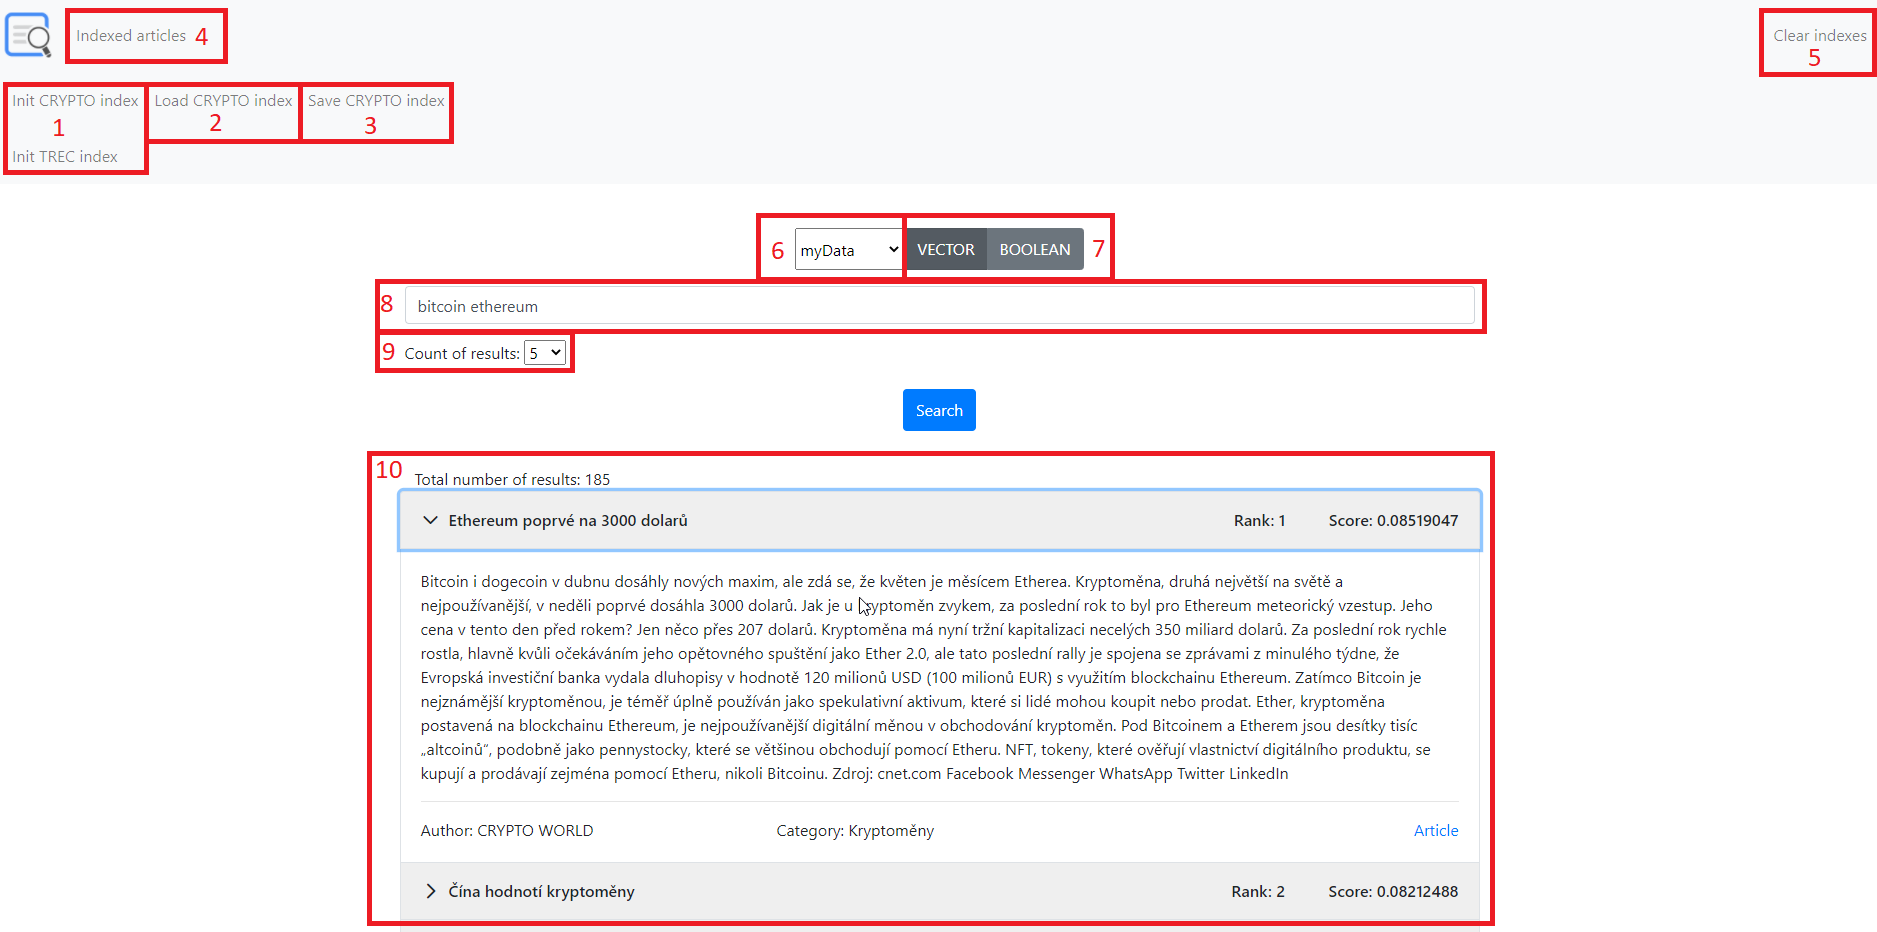
\includegraphics[width=13.5cm]{img/IR_search.png}
	\caption{Hlavní obrazovka.}
	\label{search}
\end{figure}
\begin{itemize}
    \item 1. tlačítka pro inicializaci indexů
    \begin{itemize}
        \item Init CRYPTO index - vytvoří index z dokumentů v /data/articles.json
        \item Init TREC index - vytvoří index z dat v souboru /TREC/czechData.bin
    \end{itemize}
    \item 2. tlačítko se zobrazí pokud je index uložený v souboru a lze ho načíst
    \item 3. tlačítko pro uložení seznamu z paměti aplikace do souboru
    \item 4. tlačítko pro přesun na obrazovku s výpisem zaindexovaných dokumentů (viz.\ref{article})
    \item 5. vymazání všech indexů z paměti aplikace
    \item 6. vybrání indexu, ve kterém bude aplikace hledat
    \begin{itemize}
        \item myData - index souboru articles.json
        \item trecData - index souboru czechData.bin
    \end{itemize}
    \item 7. přepínací tlačítko, určující použitý vyhledávací model
    \item 8. pole pro zadávání dotazu
    \item 9. počet zobrazených dokumentů výsledku vyhledávání
    \item 10. seznam výsledků vyhledávání
\end{itemize}
\label{article}
\section{Články}
Vysvětlení ovládacích prvků stránky se zaindexovanými články viz. obrázek \ref{articles}. Veškeré akce s články jsou prováděny nad vybraným indexem.
\begin{itemize}
    \item 1. vybrání indexu se kterým chci pracovat
    \item 2. tlačítko pro přidání článku do indexu viz. obrázek \ref{add}
    \item 3. tlačítko pro návrat na obrazovku s vyhledáváním
    \item 4. zaindexované články
    \item 5. tlačítko pro zobrazení editace článku viz. obrázek \ref{edit}
    \item 6. tlačítko pro smazání článku z indexu
\end{itemize}
\begin{figure}
    \centering
	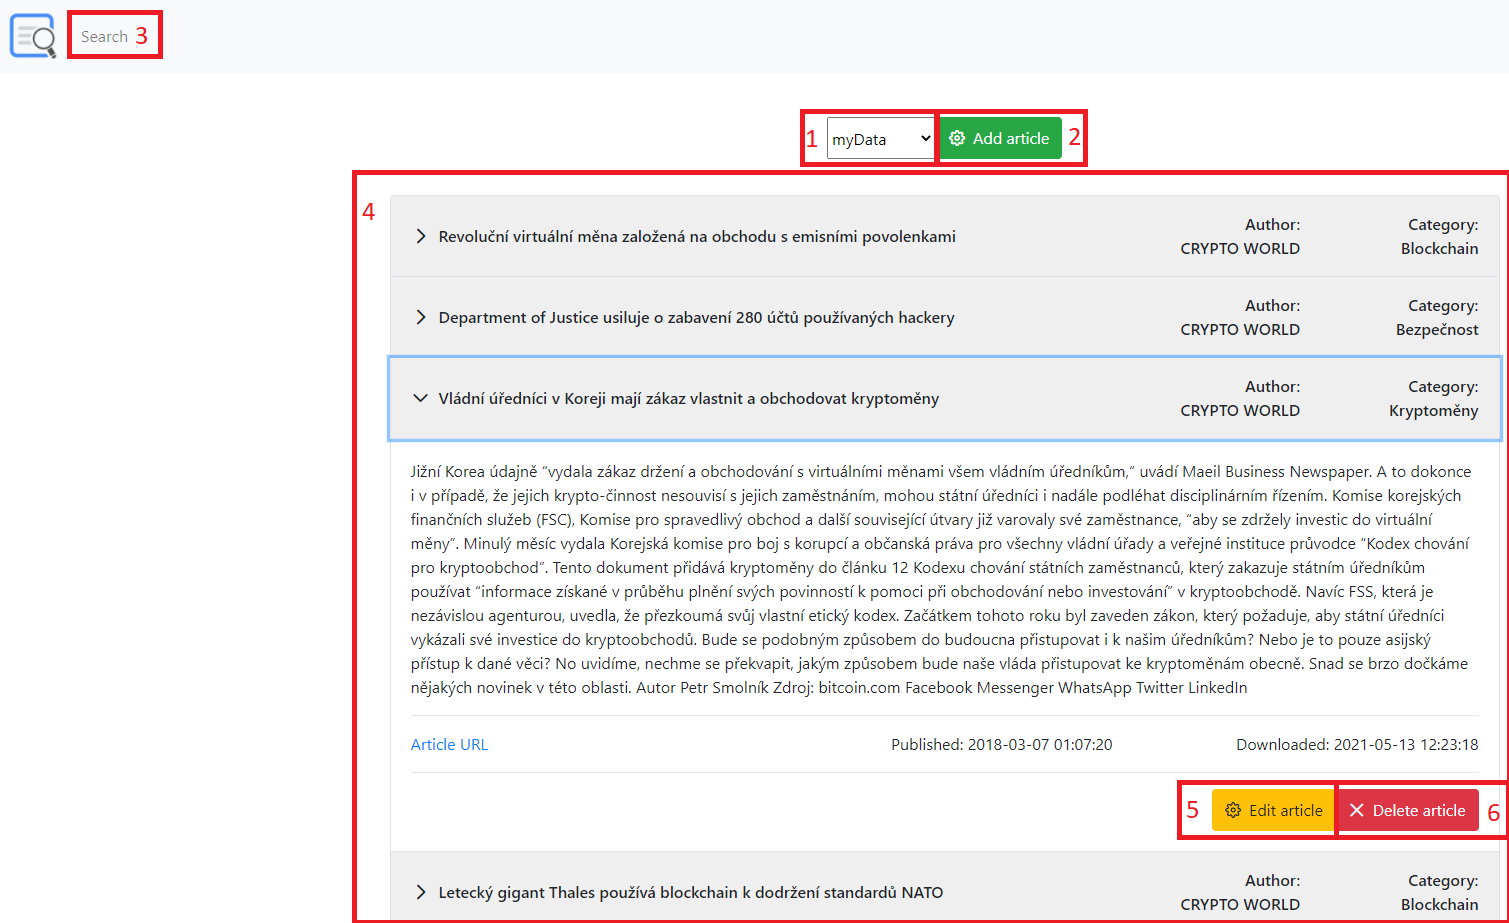
\includegraphics[width=13.5cm]{img/IR_articles.png}
	\caption{Obrazovka se zaindexovanými články.}
	\label{articles}
\end{figure}
\begin{figure}
    \centering
	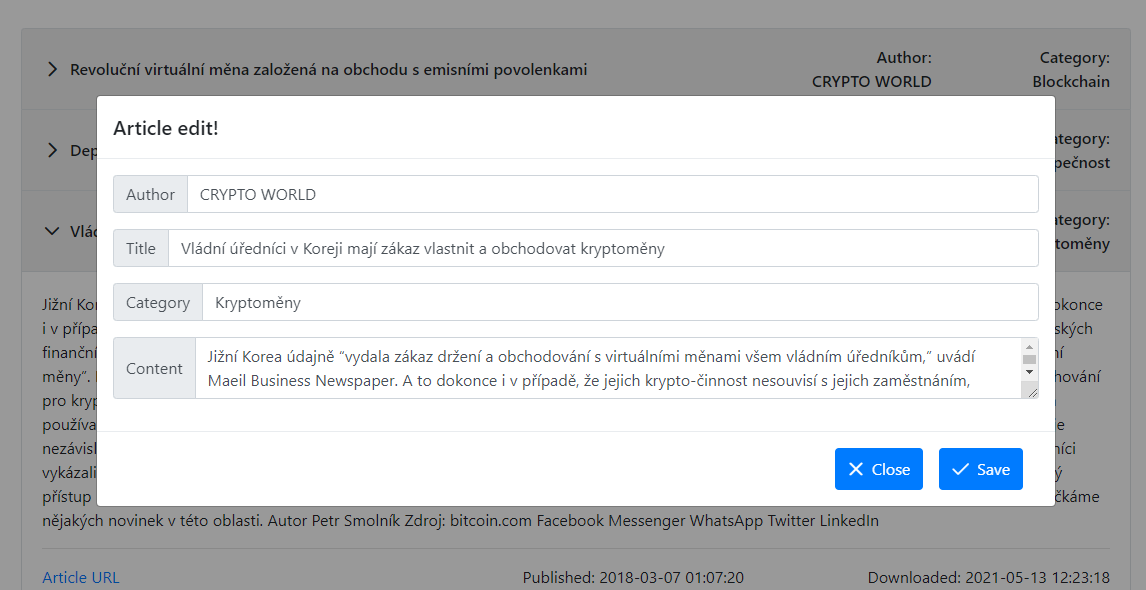
\includegraphics[width=13.5cm]{img/IR_article_edit.png}
	\caption{Úprava článku.}
	\label{edit}
\end{figure}
\begin{figure}
    \centering
	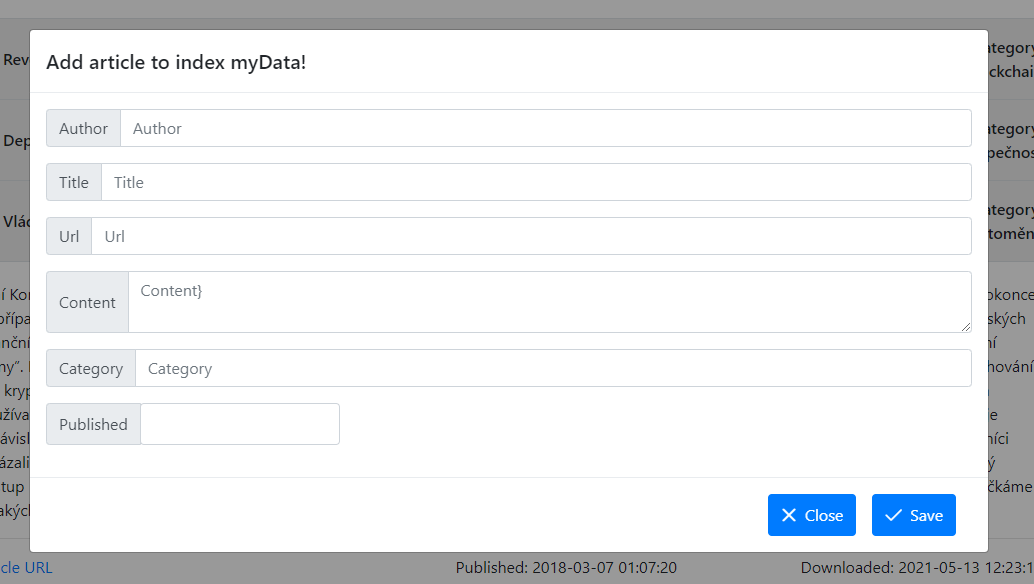
\includegraphics[width=13.5cm]{img/IR_article_add.png}
	\caption{Přidání článku.}
	\label{add}
\end{figure}
\end{document}